\chapter{Objetivos y análisis estratégico}

\section{Objetivos de la organización}

\begin{itemize}
\item Mantener un nivel de seguridad de cada operación por encima de los estándares internacionales, obteniendo una reducción de los posibles incidentes en un 2 por ciento anual.
\item Crear servicios que ayuden a la empresa a obtener mas ganancias.  
\item Contratar un experto en marketing, con por lo menos 5 años de trabajo en empresas de base tecnológica.
\item Que la empresa cuente con un servicio seguro y de calidad que sea validado por CMMI.
\item Que los precios se encuentren dentro del rango esperado por el cliente.
\item Reducir en un 2 por ciento el trafico, en la ciudad gracias a los mapas que determinaran vías alternas para movilizarse.
\end{itemize}

\section{Objetivos de marketing}

\begin{itemize}
\item Que la aplicación sea descargada por 1000 usuarios en los primeros 3 meses
\item Obtener una valoración de por lo menos 4 estrellas en la tienda de aplicaciones
\item Lograr una rentabilidad de 20 por ciento anual.
\item Alcanzar una cantidad de peticiones de 10000 a lo largo de un año.
\item Fomentar el uso de buenas practicas de manejo.
\end{itemize}

\section{Matriz FODA}

\textbf{Fortalezas}, tenemos excelentes programadores

\textbf{Debilidades}, no tenemos expertos en marketing, en contabilidad, en recursos humanos.

\textbf{Oportunidades},Se tiene la tecnología para desarrollar servicios innovadores, se cuenta con los medios de transporte existentes en la ciudad de Arequipa que podrían unirse a nuestra empresa.

\textbf{Amenazas}, la gente puede no confiar en los envíos, existe competencia, por lo que algunos obtarian por ir a otros servicios.


\begin{table}[h]
\centering
\label{tab:foda}
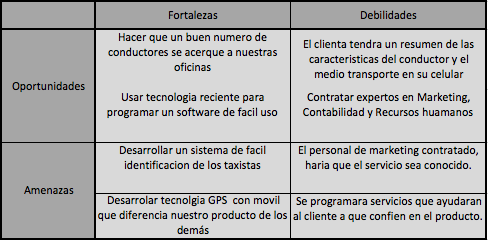
\includegraphics[width=0.8\textwidth]{TablaFODA}
\caption{Matriz FODA}
\end{table}